\documentclass[a4paper,twoside,11pt, fleqn]{article}
\usepackage{a4wide,graphicx,fancyhdr,amsmath,amssymb}
\usepackage{listings}
\usepackage{color}
\usepackage{dirtree}

%matlab 
\usepackage[]{mcode}

%----------------------- Macros and Definitions --------------------------

\setlength\headheight{20pt}
\addtolength\topmargin{-10pt}
\addtolength\footskip{20pt}

\newcommand{\N}{\mathbb{N}}
\newcommand{\ch}{\mathcal{CH}}

\newcommand{\solution}[1]{\noindent{\bf Solution to Exercise #1:}}

\fancypagestyle{plain}{%
\fancyhf{}
\fancyhead[LO,RE]{\sffamily\bfseries\large technische universiteit eindhoven}
\fancyhead[RO,LE]{\sffamily\bfseries\large 2IN35 VLSI}
\fancyfoot[LO,RE]{\sffamily\bfseries\large department of mathematics and computer science}
\fancyfoot[RO,LE]{\sffamily\bfseries\thepage}
\renewcommand{\headrulewidth}{0pt}
\renewcommand{\footrulewidth}{0pt}
}

\pagestyle{fancy}
\fancyhf{}
\fancyhead[RO,LE]{\sffamily\bfseries\large technische universiteit eindhoven}
\fancyhead[LO,RE]{\sffamily\bfseries\large 2IN35 VLSI}
\fancyfoot[LO,RE]{\sffamily\bfseries\large department of mathematics and computer science}
\fancyfoot[RO,LE]{\sffamily\bfseries\thepage}
\renewcommand{\headrulewidth}{1pt}
\renewcommand{\footrulewidth}{0pt}

\def\addsquare#1{\tikz\node[draw]{#1};} 

%-------------------------------- Title ----------------------------------

\title{\vspace{-\baselineskip}\sffamily\bfseries Assignment 4}
\author{
	Rick Veens \qquad Studentno: 0912292\\
	\texttt{r.veens@student.tue.nl}
	\and
	Barry de Bruin \qquad Studentno: 0919605\\
	\texttt{e.d.bruin@student.tue.nl}
	\and
	\texttt{Group 7}
}

\date{\today}

\setlength\parindent{0pt}

%--------------------------------- Text ----------------------------------

\begin{document}
\maketitle
\newpage

\section{Lab assignment 4a}

\subsection{Exercise 1}
\subsection{Exercise 2}
If we take for example L = 5 and M = 4, we get the following graph, while following the direct equation, we get for different y(n):

\begin{align}
y[n] &= \sum_{j=0}^3 h[j\cdot L + n\cdot M \textbf{ mod } L]\cdot x[n\cdot M \textbf{ div } L - j]\\
&= \sum_{j=0}^3 h[j\cdot 5 + n\cdot 4 \textbf{ mod } 5]\cdot x[n\cdot 4 \textbf{ div } 5 - j]
\end{align}


for n = 0 we get for j = 0 to 3:
\begin{align}
y[0] &= h[0\cdot 5 + 0\cdot 4 \textbf{ mod } 5]\cdot x[0\cdot 4 \textbf{ div } 5 - 0]\\ 
&= h[0]\cdot x[0] \\
y[0] &= h[1\cdot 5 + 0\cdot 4 \textbf{ mod } 5]\cdot x[0\cdot 4 \textbf{ div } 5 - 1] \\
&= h[5]\cdot x[-1] \\
y[0] &= h[2\cdot 5 + 0\cdot 4 \textbf{ mod } 5]\cdot x[0\cdot 4 \textbf{ div } 5 - 2] \\
&= h[10]\cdot x[-2] \\
y[0] &= h[3\cdot 5 + 0\cdot 4 \textbf{ mod } 5]\cdot x[0\cdot 4 \textbf{ div } 5 - 3] \\
&= h[15]\cdot x[-3] \\
\end{align}

for n = 1 we get for j = 0 to 3:
\begin{align}
y[1] &= h[0\cdot 5 + 1\cdot 4 \textbf{ mod } 5]\cdot x[1\cdot 4 \textbf{ div } 5 - 0]]\\ 
&= h[4]\cdot x[0] \\
y[1] &= h[1\cdot 5 + 1\cdot 4 \textbf{ mod } 5]\cdot x[1\cdot 4 \textbf{ div } 5 - 1]] \\
&= h[9]\cdot x[-1] \\
y[1] &= h[2\cdot 5 + 1\cdot 4 \textbf{ mod } 5]\cdot x[1\cdot 4 \textbf{ div } 5 - 2]] \\
&= h[14]\cdot x[-2] \\
y[1] &= h[3\cdot 5 + 1\cdot 4 \textbf{ mod } 5]\cdot x[1\cdot 4 \textbf{ div } 5 - 3]] \\
&= h[19]\cdot x[-3] \\
\end{align}

for n = 2 we get for j = 0 to 3:
\begin{align}
y[1] &= h[0\cdot 5 + 2\cdot 4 \textbf{ mod } 5]\cdot x[2\cdot 4 \textbf{ div } 5 - 0]]\\ 
&= h[3]\cdot x[1] \\
y[1] &= h[1\cdot 5 + 2\cdot 4 \textbf{ mod } 5]\cdot x[2\cdot 4 \textbf{ div } 5 - 1]] \\
&= h[8]\cdot x[0] \\
y[1] &= h[2\cdot 5 + 2\cdot 4 \textbf{ mod } 5]\cdot x[2\cdot 4 \textbf{ div } 5 - 2]] \\
&= h[13]\cdot x[-1] \\
y[1] &= h[3\cdot 5 + 2\cdot 4 \textbf{ mod } 5]\cdot x[2\cdot 4 \textbf{ div } 5 - 3]] \\
&= h[18]\cdot x[-2] \\
\end{align}

for n = 3 we get for j = 0 to 3:
\begin{align}
y[1] &= h[0\cdot 5 + 3\cdot 4 \textbf{ mod } 5]\cdot x[3\cdot 4 \textbf{ div } 5 - 0]]\\ 
&= h[2]\cdot x[2] \\
y[1] &= h[1\cdot 5 + 3\cdot 4 \textbf{ mod } 5]\cdot x[3\cdot 4 \textbf{ div } 5 - 1]] \\
&= h[7]\cdot x[1] \\
y[1] &= h[2\cdot 5 + 3\cdot 4 \textbf{ mod } 5]\cdot x[3\cdot 4 \textbf{ div } 5 - 2]] \\
&= h[12]\cdot x[0] \\
y[1] &= h[3\cdot 5 + 3\cdot 4 \textbf{ mod } 5]\cdot x[3\cdot 4 \textbf{ div } 5 - 3]] \\
&= h[17]\cdot x[-1] \\
\end{align}

for n = 4 we get for j = 0 to 3:
\begin{align}
y[1] &= h[0\cdot 5 + 4\cdot 4 \textbf{ mod } 5]\cdot x[4\cdot 4 \textbf{ div } 5 - 0]]\\ 
&= h[1]\cdot x[3] \\
y[1] &= h[1\cdot 5 + 4\cdot 4 \textbf{ mod } 5]\cdot x[4\cdot 4 \textbf{ div } 5 - 1]] \\
&= h[6]\cdot x[2] \\
y[1] &= h[2\cdot 5 + 4\cdot 4 \textbf{ mod } 5]\cdot x[4\cdot 4 \textbf{ div } 5 - 2]] \\
&= h[11]\cdot x[1] \\
y[1] &= h[3\cdot 5 + 4\cdot 4 \textbf{ mod } 5]\cdot x[4\cdot 4 \textbf{ div } 5 - 3]] \\
&= h[16]\cdot x[0] \\
\end{align}

Now it starts repeating:\\

for n = 5 we get for j = 0 to 3:
\begin{align}
y[1] &= h[0\cdot 5 + 5\cdot 4 \textbf{ mod } 5]\cdot x[5\cdot 4 \textbf{ div } 5 - 0]]\\ 
&= h[0]\cdot x[0] \\
y[1] &= h[1\cdot 5 + 5\cdot 4 \textbf{ mod } 5]\cdot x[5\cdot 4 \textbf{ div } 5 - 1]] \\
&= h[5]\cdot x[-1] \\
y[1] &= h[2\cdot 5 + 5\cdot 4 \textbf{ mod } 5]\cdot x[5\cdot 4 \textbf{ div } 5 - 2]] \\
&= h[10]\cdot x[-2] \\
y[1] &= h[3\cdot 5 + 5\cdot 4 \textbf{ mod } 5]\cdot x[5\cdot 4 \textbf{ div } 5 - 3]] \\
&= h[15]\cdot x[-3] \\
\end{align}


\newpage
\subsection{Exercise 3}
We have the following 4 designs: 

\subsubsection{Direct equation solution}
This solution uses the direct equation and has two different implementations: The direct method that has a single direct equation stage, and the composite implementation that uses two stages.

\smallskip
\textbf{Direct method}\\
This implementation uses $4\cdot L$ coefficients and needs only 4 multiplications/additions. All inner factors can be pre-computed.
\smallskip
The highest sample rate inside the system (system frequency) will be input or output sample frequency, depending on the L and M constants. Therefore: $F_{system} = max(Fs_{in}, Fs_{out})$.
 
\smallskip 
\textbf{Composite method}\\
Uses $4\cdot (L_{sub1} + L_{sub2})$ coefficients, while $L = L_{sub1} \cdot L_{sub2}$. Therefore we need less coefficients compared to the direct method. Since every sample still needs 4 multiplications/additions, we actually need 8 multiplication/additions for this implementation.

\smallskip
If we compose a resampler of two of those systems, the highest system frequency will be input frequency of the first system, the output of the first system (input of second system), or the output of the second system.

\subsubsection{Naive solution}
Uses the complete part of an upscaler, low-pass filter and downscaler. Again we have two variants:

\smallskip
\textbf{Direct scalers}\\
Since the filter in this implementation is just a low-pass FIR filter, we need one multiplication/addition step for every coefficient. This is not very efficient because L-1 out of L samples are zero and will therefore not influence the output signal. Because $4\cdot L$ coefficients are needed to filter out the high-frequency noise, we need the same amount of multiplication/additions for one output sample.

\smallskip
The maximum system frequency will be $F_{system} = F_s\cdot L$ Hz, which is the sampling frequency of the low-pass filter. This is also shown in figure xx below:
\begin{figure}[h]
	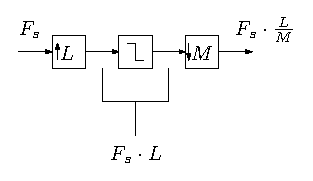
\includegraphics[scale = 1]{Images/3_0}
    \caption{Naive solution with single set of stages}
\end{figure}

\newpage
\textbf{Composite scalers } \\
Now we actually have two stages and therefore we need to apply the FIR filter in both stages. This will actually cost us $4\cdot (L_1 + L_2)$ multiplication/addition steps, where still L-1 out of L samples are zero.

\smallskip
The maximum system frequency will be $F_{system} = max(F_s\cdot L_1, F_s\cdot \frac{L_1\cdot L_2}{M_1})$, since one of the two stages can have the highest frequency, depending on the L and M parameters.
\begin{figure}[h]
	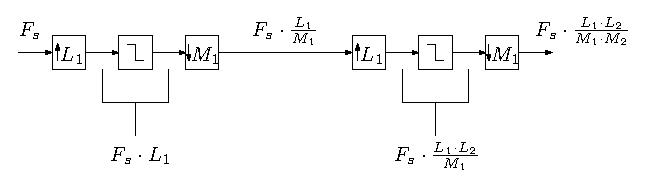
\includegraphics[scale = 1]{Images/3_1}
    \caption{Naive solution with double set of stages}
\end{figure}

\subsubsection{Conclusion}
The best solution may depend on your needs. If your L is really large, we may consider using a composite solution to exchange coefficient memory for additional arithmetic steps. The naive method does make a lot of useless computations, while the direct equation method has almost no computations with a zero factor.\\

Therefore we can say that for our upsampler, the single-stage direct equation solution is best, since we only have to store 160 coefficients, and still can get maximum performance of doing only 4 multiplications/additions per sample.

\newpage
\subsection{Implementation}
Since input frequency is only 44khz, and output frequency only 48khz, we can just implement this by using a single DSP unit.\\

I generate the coefficients using matlab. They are in the coef.bin file, and already multiplied by $2^{16}$ and rounded.\\

If the lanczos2 function gives a close to one output, the quantized value will be close to the maximum that a 16-bit value can hold. Therefore 16-bit is not enough to store the summation and multiplication of multiple of such values.\\

\begin{lstlisting}
% Put this in a file named coef_generate_matlab.m, 
% then call it while you are in the file directory


function [y] = coef_generate_matlab(L)
        % make sure that coefficients sum to 1
        y = coef_gen(L);
        y = coef_gen(L)/sum(y);

        % quantize and round to nearest integer
        y = round(y*(2^16)); 
             
        % convert to signed int filter coeff
        y = int16(y);
        y = hex(fi(y, 1, 16, 0)); %1 stands for signed, 16 bit out
        y= y(~isspace(y)); % remove spaces
        dlmwrite('coef.txt',y,''); %create file, with no delimiter ''      
end

function [y] = coef_gen(L)
    % generate 4*L coefficients and start at 0 instead of 1 *stupid matlab*
    for n = 1:4*L
            y(n) = lanczos2(((n-1)/L) -2);
    end
end

function y = lanczos2(t)
    if(t <= -2 || t >= 2)
        y = 0;
    else
        y = sinc(t).*sinc(t/2);
    end
end

%%



\end{lstlisting}


\end{document}
